\documentclass{article}
\usepackage[a4paper, 
            left=1in, 
            right=1.25in, 
            top=0.9in, 
            bottom=1in]{geometry}
\usepackage{vntex}
\usepackage{graphicx}
\usepackage{float}
\usepackage{hyperref}
\usepackage{amsmath}
\usepackage{amssymb}
\usepackage{xcolor}
\usepackage{array}
\usepackage{multirow}
\usepackage{caption}
\usepackage{tabularx}
\usepackage{longtable}
\hypersetup{
    colorlinks=true,
    linkcolor=red,
    filecolor=magenta,      
    urlcolor=cyan,
    pdftitle={Overleaf},
    pdfpagemode=FullScreen,
}
\usepackage{fancyhdr}
\pagestyle{fancy}
% \usepackage{atveryend}
\usepackage{parskip}
% \usepackage[vietnamese]{babel}
\fancyhf{}
\fancyhead[L]{
 \begin{tabular}{rl}
    \begin{picture}(25,15)(0,0)
    \put(0,-8){
\includegraphics[width=8mm, height=8mm]{img/hcmut.png}}
   \end{picture}&
	\begin{tabular}{l}
		\textbf{\bf \ttfamily Trường Đại học Bách Khoa}\\
		\textbf{\bf \ttfamily Khoa Khoa học và Kỹ thuật Máy tính} 
	\end{tabular} 	
 \end{tabular}
}

\fancyfoot[L]{\scriptsize \ttfamily Đồ án Tổng hợp - hướng Công nghệ Phần mềm (CO3103), Học kỳ 1, Năm học 2025 - 2026}

\renewcommand{\headrulewidth}{0.1pt}
\renewcommand{\footrulewidth}{0.1pt}

\AtBeginDocument{\renewcommand*\contentsname{Mục lục}}
\AtBeginDocument{\renewcommand{\listfigurename}{Danh sách hình ảnh}}
\AtBeginDocument{\renewcommand{\listtablename}{Danh sách bảng biểu}}
\AtBeginDocument{\renewcommand*\refname{Tài liệu tham khảo}}

\begin{document}
\begin{titlepage}
\begin{center}
ĐẠI HỌC QUỐC GIA TP. HỒ CHÍ MINH\\
TRƯỜNG ĐẠI HỌC BÁCH KHOA\\
KHOA KHOA HỌC VÀ KỸ THUẬT MÁY TÍNH
\end{center}

\begin{figure}[h!]
\begin{center}

\includegraphics[width=3cm]{img/hcmut.png}
\end{center}
\end{figure}

\centering
\LARGE\textbf{Đồ án Tổng hợp - hướng Công nghệ Phần mềm} \\
\LARGE\textbf{(CO3103)} 

\begin{center}
\rule{14cm}{0.1pt}
\vspace{0.2cm} \\
    \vspace{0.5cm}
    \textbf{\textit{{\Huge Second Hand Land}}} \\
    \vspace{0.5cm}
    \rule{14cm}{0.1pt}
\end{center}

\vspace{0.5cm}
\begin{table}[h]
\centering
\begin{tabular}{l l l l}
    \textbf{GVHD}:      & Mai Đức Trung   &          &     \\  [3pt]
    \textbf{Nhóm}:      & UIA             &          &     \\  [3pt]
    \textbf{Sinh viên}: & Nguyễn Trung An & 2310027  & L04 \\
                        & Hồ Thị Minh Thu & 2313342  & L04 \\
                        & Phan Hoàng Kiên & 2311741  & L04 \\
                        & Lê Quốc Kiệt    & 2311767  & L04 \\
                        & Trần Gia Kiệt   & 2311784  & L04 \\
\end{tabular}
\end{table}
\vspace{9cm}
\centering

\small TP. Hồ Chí Minh, Tháng 9 năm 2025
\end{titlepage}
\newpage
\fancyfoot[R]{\scriptsize \ttfamily Trang {\thepage}/\pageref{LastPageArabic}}

\newpage
\section{Tổng Quan Dự Án}
\subsection{Thực Trạng}

\quad Trong những năm gần đây, nhu cầu trao đổi và mua bán đồ cũ ngày càng tăng, phản ánh xu hướng tiêu dùng bền vững và tiết kiệm chi phí của xã hội hiện đại. Người dùng không chỉ tìm kiếm các sản phẩm có giá trị sử dụng tốt với chi phí hợp lý, mà còn mong muốn góp phần giảm thiểu rác thải, bảo vệ môi trường thông qua việc tái sử dụng.

\quad Tuy nhiên, các nền tảng giao dịch đồ cũ hiện nay như Chợ Tốt, Carousell hay eBay vẫn còn tồn tại một số hạn chế nhất định. Các vấn đề phổ biến bao gồm: thiếu cơ chế minh bạch trong giao dịch, rủi ro về lừa đảo, thiếu sự gắn kết cộng đồng, và ít chú trọng đến việc khuyến khích người dùng tham gia lâu dài. Bên cạnh đó, trải nghiệm người dùng thường chỉ dừng lại ở mức kết nối người mua và người bán, chưa tạo ra được hệ sinh thái mua bán bền vững xoay quanh hành vi tái sử dụng.

\quad Trong bối cảnh đó, dự án Second Hand Land được đề xuất như một giải pháp nhằm giải quyết những hạn chế hiện hữu, đồng thời mở ra hướng tiếp cận mới mẻ trong việc xây dựng một cộng đồng mua bán, trao đổi đồ cũ an toàn, minh bạch, và có tính kết nối cao.  
\subsection{Mô Tả Dự Án} 
\quad Second Hand Land là một nền tảng trực tuyến cho phép người dùng mua, bán hoặc trao đổi đồ dùng đã qua sử dụng. Điểm khác biệt cốt lõi của hệ thống nằm ở việc kết hợp song song hai cơ chế thanh toán: bằng tiền và bằng điểm tích lũy (point-based system). Cơ chế này vừa khuyến khích hành vi tái sử dụng, vừa tạo động lực gắn bó lâu dài của người dùng thông qua việc tích lũy, đổi điểm, tham gia sự kiện và chương trình cộng đồng.

\quad Bên cạnh yếu tố giao dịch, hệ thống cũng chú trọng đến việc xây dựng một cộng đồng gắn kết thông qua hoạt động thiện nguyện, minigame, hoặc sự kiện khuyến mãi. Đây là một yếu tố tạo sự khác biệt so với các nền tảng mua bán đồ cũ truyền thống, khi người dùng không chỉ đơn thuần tham gia giao dịch, mà còn được trải nghiệm một môi trường mang tính xã hội và cộng đồng cao hơn. Hệ thống cũng dự kiến sẽ tích hợp với các dịch vụ bên ngoài thông qua API (xác thực tài khoản, thanh toán điện tử, dịch vụ vận chuyển) để đảm bảo an toàn, minh bạch và tối ưu trải nghiệm người dùng.

\subsection{Mục Tiêu Dự Án}
Dự án hướng tới các mục tiêu chính sau:
\begin{itemize}
    \item Xây dựng nền tảng minh bạch, an toàn: hạn chế rủi ro lừa đảo, nâng cao độ tin cậy trong giao dịch đồ cũ.
    \item Khuyến khích hành vi tái sử dụng: góp phần giảm lãng phí, bảo vệ môi trường và thúc đẩy lối sống xanh.
    \item Tạo cơ chế khuyến khích cộng đồng: thông qua hệ thống điểm, sự kiện và các chương trình gắn kết để duy trì động lực sử dụng lâu dài.
    \item Mở rộng hệ sinh thái: thông qua việc tích hợp với các đối tác (thanh toán, vận chuyển, xác thực) để mang lại trải nghiệm liền mạch cho người dùng.  
\end{itemize}

\subsection{Đối tượng người dùng}

\begin{itemize}
    \item Cá nhân: những người có nhu cầu mua bán, trao đổi đồ cũ nhằm tiết kiệm chi phí hoặc tìm kiếm sản phẩm đặc thù.
    \item Sinh viên và người lao động trẻ: nhóm có thu nhập hạn chế, thường xuyên tìm kiếm các lựa chọn tiết kiệm và có xu hướng quan tâm đến cộng đồng.

    \item Người tiêu dùng quan tâm môi trường: mong muốn tham gia các hoạt động tái sử dụng để giảm tác động tiêu cực đến môi trường.
    \item Người bán chuyên nghiệp nhỏ lẻ: những cá nhân/hộ kinh doanh muốn tận dụng nền tảng để bán hàng cũ hoặc hàng tồn kho.
\end{itemize}

\subsection{Các Bên Liên Quan}

\begin{itemize}
    \item Người dùng: khách hàng cá nhân vừa là người mua vừa là người bán. Đây là đối tượng trung tâm quyết định sự thành công của hệ thống.
    \item Quản trị viên: chịu trách nhiệm giám sát nền tảng, kiểm duyệt nội dung, xử lý báo cáo vi phạm, quản lý sự kiện và duy trì tính ổn định của hệ thống.
    \item Đối tác bên ngoài: bao gồm đơn vị cung cấp dịch vụ thanh toán, đơn vị vận chuyển và dịch vụ xác thực. Các bên này đóng vai trò quan trọng trong việc tạo sự tin cậy và hoàn thiện trải nghiệm giao dịch.
    \item Cộng đồng: ngoài người dùng trực tiếp, còn có các tổ chức xã hội, nhóm thiện nguyện hoặc các chương trình môi trường hợp tác để tạo ra giá trị chung.
\end{itemize}

\subsection{Ý Nghĩa và Giá Trị Kỳ Vọng}

\begin{itemize}
    \item Giảm thiểu rác thải và khuyến khích tái sử dụng: tạo ra một vòng tuần hoàn giá trị cho các sản phẩm cũ.

    \item Tăng cường sự tin cậy trong giao dịch trực tuyến: thông qua minh bạch hóa quy trình và tích hợp dịch vụ an toàn.
    \item Xây dựng cộng đồng gắn kết: nơi người dùng không chỉ tham gia giao dịch mà còn tương tác, chia sẻ và đóng góp cho xã hội.
    \item Mở ra cơ hội kinh doanh mới: cho các cá nhân và hộ kinh doanh nhỏ lẻ muốn tận dụng nền tảng để mở rộng thị trường.
\end{itemize}

\section{Phân Tích Yêu Cầu}
\subsection{Yêu Cầu Chức Năng}
\subsection*{Đối với Customer}
\subsubsection*{1. Quản lý tài khoản}
\begin{itemize}
    \item Hệ thống cho phép người dùng đăng ký tài khoản mới bằng email/số điện thoại và mật khẩu.
    \item Hệ thống hỗ trợ xác thực danh tính người dùng thông qua OTP/email hoặc dịch vụ xác thực bên ngoài.
    \item Người dùng có thể đăng nhập, đăng xuất, và khôi phục mật khẩu qua email/số điện thoại.
    \item Người dùng có thể chỉnh sửa thông tin cá nhân (tên, địa chỉ, số điện thoại, email, mật khẩu).
\end{itemize}

\subsubsection*{2. Xem \& Tìm kiếm sản phẩm}
\begin{itemize}
    \item Người dùng có thể tìm kiếm sản phẩm theo từ khóa, loại, giá, điểm, tình trạng, vị trí.
    \item Người dùng có thể xem chi tiết sản phẩm (hình ảnh, mô tả, giá điểm, thông tin người bán).
    \item Hệ thống cung cấp tính năng gợi ý sản phẩm dựa trên lịch sử mua/bán và hành vi duyệt sản phẩm.
    \item Người dùng có thể thêm sản phẩm vào giỏ hàng, wishlist để theo dõi sau.

\end{itemize}

\subsubsection*{3. Mua hàng \& thanh toán}
\begin{itemize}
    \item Người mua có thể áp dụng voucher/mã giảm giá vào đơn hàng.
    \item Người mua có thể thanh toán bằng điểm, tiền mặt (nạp qua cổng thanh toán), hoặc kết hợp cả hai.
    \item Người mua có thể đổi điểm sang tiền theo tỷ lệ quy định.
    \item Hệ thống gửi thông báo trạng thái thanh toán (thành công/thất bại).
\end{itemize}

\subsubsection*{4. Lịch sử đơn hàng}
\begin{itemize}
    \item Người dùng có thể xem lịch sử mua/bán hàng (đơn đã đặt, đang xử lý, đã giao, đã hủy).
    \item Người dùng có thể đánh giá và phản hồi về sản phẩm và người bán sau khi nhận hàng.
    \item Người dùng có thể yêu cầu trả hàng hoặc hủy đơn (theo chính sách).

    \item Hệ thống cập nhật trạng thái đơn hàng theo dịch vụ Delivery.
\end{itemize}

\subsubsection*{5. Đăng \& Quản lý sản phẩm}
\begin{itemize}
    \item Người bán có thể đăng sản phẩm mới (hình ảnh, mô tả, giá).
    \item Người bán có thể chỉnh sửa, ẩn hoặc xóa sản phẩm đã đăng.
    \item Hệ thống hỗ trợ kiểm duyệt (tự động hoặc qua admin) trước khi sản phẩm hiển thị công khai.
    \item Người bán có thể theo dõi trạng thái sản phẩm (đang chờ duyệt, đang hiển thị, đã bán).
\end{itemize}

\subsubsection*{6. Xử lí đơn hàng}
\begin{itemize}

    \item Người bán nhận thông báo khi có đơn hàng mới.

    \item Hệ thống xử lý tình trạng đơn hàng (chờ xác nhận, đang giao, hoàn tất).

    \item Người bán có thể cập nhật tình trạng đơn hàng.
    
    \item Khi hệ thống nhận được thông báo từ Delivery rằng đơn hàng đã giao thành công, hệ thống sẽ chuyển từ tài khoản tạm giữ (escrow) của hệ thống sang ví của người bán.

\end{itemize}

\subsubsection*{7. Tham gia sự kiện}
\begin{itemize}
    \item Người dùng có thể tham gia các sự kiện (khuyến mãi, đấu giá, flash sale).

    \item Hệ thống hiển thị thông tin sự kiện và áp dụng ưu đãi khi mua hàng.
\end{itemize}

\subsubsection*{8. Yêu cầu hỗ trợ}
\begin{itemize}
    \item Người dùng có thể gửi yêu cầu hỗ trợ (qua chat, email hoặc ticket).

    \item Hệ thống ghi nhận và phản hồi từ bộ phận hỗ trợ.
\end{itemize}

\subsubsection*{9. Quản lý số dư \& điểm }


\begin{itemize}

    \item Người dùng có thể quy đổi tiền sang điểm hoặc ngược lại theo tỷ lệ quy định để sử dụng khi mua hàng.
    \item Hệ thống cập nhật số dư ví và điểm của người dùng sau mỗi giao dịch.
    \item Người dùng có thể xem lịch sử giao dịch (nạp tiền, rút tiền, quy đổi).
\end{itemize}

\subsection*{Đối với Admin}

\subsubsection*{1. Tổ chức sự kiện}
\begin{itemize}
    \item Admin có thể tạo/sửa/xóa sự kiện (flash sale, khuyến mãi).
    \item Hệ thống áp dụng sự kiện theo thời gian và điều kiện do admin cài đặt.
\end{itemize}

\subsubsection*{2. Hỗ trợ khách hàng}
\begin{itemize}
    \item Admin có thể tiếp nhận và phản hồi yêu cầu hỗ trợ từ khách hàng.
    \item Hệ thống ghi nhận tình trạng xử lý (đang chờ, đã xử lý).
\end{itemize}

\subsubsection*{3. Kiểm duyệt}
\begin{itemize}
    \item Admin có thể duyệt, từ chối hoặc xóa sản phẩm người dùng đăng.
    \item Admin có thể khóa tài khoản vi phạm chính sách.
    \item Admin có thể theo dõi hoạt động giao dịch bất thường.
\end{itemize}
\subsubsection*{4. Phân tích dữ liệu}
\begin{itemize}
    \item Admin có thể xem báo cáo tổng quan (số lượng giao dịch, doanh thu, lượng người dùng).
    \item Admin có thể xem phân tích xu hướng sản phẩm (mặt hàng bán chạy, giá phổ biến).
    \item Hệ thống xuất báo cáo định kỳ.
\end{itemize}

\subsection{Yêu Cầu Phi Chức Năng}

\subsubsection*{1. Hiệu năng}
\begin{itemize}
    \item Hệ thống phải xử lý ít nhất 1000 request/giây ở giờ cao điểm.
    \item Thời gian phản hồi trung bình của một request không vượt quá 2 giây.
    \item Hệ thống hỗ trợ ít nhất 10.000 người dùng trực tuyến đồng thời mà không gián đoạn dịch vụ.
\end{itemize}

\subsubsection*{2. Khả năng mở rộng}
\begin{itemize}
    \item Hệ thống phải dễ dàng mở rộng để xử lý gấp 5 lần lượng người dùng hiện tại mà không cần thay đổi kiến trúc lõi.
\end{itemize}

\subsubsection*{3. Bảo mật}
\begin{itemize}
    \item Tất cả dữ liệu nhạy cảm (mật khẩu, thông tin thanh toán) phải được mã hóa bằng AES-256.
    \item Hệ thống phải hỗ trợ 2FA (xác thực hai lớp) cho tài khoản người dùng.
    \item Hệ thống phải đạt chuẩn OWASP Top 10 để phòng chống tấn công (SQL injection, XSS, CSRF…).
\end{itemize}

\subsubsection*{4. Tính sẵn sàng \& tin cậy}
\begin{itemize}
    \item Hệ thống phải đạt uptime $\geq 99.5\%$/tháng.
    \item Trong trường hợp sự cố, dữ liệu phải được khôi phục trong vòng $< 30$ phút từ bản backup gần nhất.
    \item Hệ thống phải thực hiện backup dữ liệu hằng ngày và lưu giữ ít nhất 30 ngày gần nhất.
\end{itemize}

\subsubsection*{5. Trải nghiệm người dùng}
\begin{itemize}
    \item Trang sản phẩm phải tải trong vòng $\leq 3$ giây kể cả khi có 1000 ảnh sản phẩm đang hiển thị.
    \item Giao diện trực quan và dễ sử dụng trên cả desktop, tablet, mobile, với độ tương thích $\geq 95\%$ trên các trình duyệt phổ biến: Chrome ($\geq 90$), Edge ($\geq 90$), Safari ($\geq 15$), Firefox ($\geq 90$).
\end{itemize}

\subsubsection*{6. Khả năng bảo trì}
\begin{itemize}
    \item Mã nguồn phải tuân thủ coding convention thống nhất và được tài liệu hóa.
    \item Thời gian sửa lỗi nghiêm trọng (critical bug) không vượt quá 24 giờ kể từ khi phát hiện.
\end{itemize}

\subsubsection*{7. Khả năng giám sát}
\begin{itemize}
    \item Hệ thống phải cung cấp dashboard giám sát realtime (số lượng người dùng online, giao dịch, đơn hàng).
    \item Log giao dịch và log lỗi phải được lưu giữ ít nhất 90 ngày để phục vụ kiểm tra gian lận.
    \
\end{itemize}
\section{Nghiên Cứu và Lựa Chọn Công Nghệ}

\subsection{Frontend Framework}

\textbf{Angular}
\begin{itemize}
    \item Ưu điểm: Mạnh, đầy đủ tính năng, chuẩn MVVM.
    \item Nhược điểm: Khá phức tạp, học lâu, dung lượng lớn.
\end{itemize}

\textbf{VueJS}
\begin{itemize}
    \item Ưu điểm: Dễ học, code gọn, cộng đồng ngày càng phát triển.
    \item Nhược điểm: Ít thư viện doanh nghiệp hỗ trợ hơn React.
\end{itemize}

\textbf{ReactJS}
\begin{itemize}
    \item Ưu điểm: Phổ biến nhất hiện nay, thư viện UI phong phú, cộng đồng lớn, dễ tích hợp backend.
    \item Nhược điểm: Chỉ là thư viện, cần thêm các package để hoàn thiện (routing, state management).
\end{itemize}

\textbf{Lựa chọn:} ReactJS vì phổ biến, dễ mở rộng và tối ưu cho ứng dụng web có UI phức tạp.

\subsection{Backend Framework}

\textbf{Django (Python)}
\begin{itemize}
    \item Ưu điểm: Hệ sinh thái lớn, tích hợp sẵn nhiều module (auth, admin), bảo mật cao.
    \item Nhược điểm: Ít linh hoạt khi tùy biến API, cú pháp phức tạp hơn, hosting tốn chi phí hơn Node.js.
\end{itemize}

\textbf{Spring Boot (Java)}
\begin{itemize}
    \item Ưu điểm: Độ tin cậy cao, phù hợp cho hệ thống quy mô lớn, hỗ trợ microservices tốt.
    \item Nhược điểm: Khó học, nặng, tốn nhiều tài nguyên.
\end{itemize}

\textbf{Express (Node.js)}
\begin{itemize}
    \item Ưu điểm: Nhẹ, linh hoạt, phổ biến, nhiều package npm, dễ xây dựng API RESTful.
    \item Nhược điểm: Yêu cầu lập trình viên quản lý nhiều thứ thủ công (bảo mật, cấu trúc).
\end{itemize}

\textbf{Lựa chọn:} Express.js vì tính nhẹ, linh hoạt, cộng đồng lớn và phù hợp với quy mô dự án marketplace.

\subsection{UI/UX Design}
\textbf{Figma}
\begin{itemize}
    \item Ưu điểm: Làm việc nhóm trực tuyến thời gian thực, miễn phí cho nhóm nhỏ, kho plugin phong phú, dễ chia sẻ.
    \item Nhược điểm: Phụ thuộc vào kết nối Internet, bản offline hạn chế.
\end{itemize}

\textbf{Adobe XD}
\begin{itemize}
    \item Ưu điểm: Giao diện trực quan, hỗ trợ prototyping nhanh.
    \item Nhược điểm: Cộng đồng nhỏ hơn Figma, ít plugin.
\end{itemize}

\textbf{Sketch}
\begin{itemize}
    \item Ưu điểm: Mạnh về thiết kế vector, nhiều plugin.
    \item Nhược điểm: Chỉ hỗ trợ macOS, không làm việc nhóm trực tuyến tốt.
\end{itemize}

\textbf{Lựa chọn:} Figma vì hỗ trợ cộng tác thời gian thực, dễ dùng, phù hợp với sinh viên và đội nhóm phát triển web.

\subsection{Database}

\textbf{MySQL}
\begin{itemize}
    \item Ưu điểm: Ổn định, phổ biến, dễ triển khai.
    \item Nhược điểm: Cứng nhắc với dữ liệu không có cấu trúc.
\end{itemize}

\textbf{PostgreSQL}
\begin{itemize}
    \item Ưu điểm: Chuẩn ACID, mạnh về dữ liệu phức tạp.
    \item Nhược điểm: Cấu hình phức tạp hơn MySQL.
\end{itemize}

\textbf{MongoDB}
\begin{itemize}
    \item Ưu điểm: Lưu trữ dữ liệu theo dạng JSON, linh hoạt cho sản phẩm/đơn hàng/user, dễ mở rộng.
    \item Nhược điểm: Không mạnh bằng SQL trong các truy vấn phức tạp.
\end{itemize}

\textbf{Lựa chọn:} MongoDB vì cấu trúc dữ liệu linh hoạt, phù hợp với hệ thống thương mại điện tử nơi sản phẩm có nhiều thuộc tính khác nhau.

\subsection{Authentication}

\textbf{Session-based Authentication}
\begin{itemize}
    \item Ưu điểm: Dễ triển khai, truyền thống.
    \item Nhược điểm: Không phù hợp với API stateless.
\end{itemize}

\textbf{OAuth2.0}
\begin{itemize}
    \item Ưu điểm: Chuẩn công nghiệp, hỗ trợ login Google/Facebook.
    \item Nhược điểm: Cấu hình phức tạp hơn.
\end{itemize}

\textbf{JSON Web Token (JWT)}
\begin{itemize}
    \item Ưu điểm: Phù hợp với API RESTful, nhẹ, dễ tích hợp.
    \item Nhược điểm: Khó thu hồi token trước khi hết hạn.
\end{itemize}

\textbf{Lựa chọn:} JWT vì gọn nhẹ, phù hợp với kiến trúc frontend-backend tách biệt.


\subsection{Testing}

\textbf{Jest (JavaScript/TypeScript)}
\begin{itemize}
    \item Ưu điểm: Hỗ trợ tốt cho React và Node.js, phổ biến, dễ tích hợp CI/CD.
    \item Nhược điểm: Có thể chậm với test phức tạp.
\end{itemize}

\textbf{Cypress}
\begin{itemize}
    \item Ưu điểm: Mạnh về end-to-end (E2E), mô phỏng hành vi thực tế người dùng trên giao diện web.
    \item Nhược điểm: Test phức tạp có thể chạy chậm.
\end{itemize}

\textbf{Selenium}
\begin{itemize}
    \item Ưu điểm: Truyền thống, đa ngôn ngữ, phù hợp test cross-browser.
    \item Nhược điểm: Cồng kềnh, cần nhiều tài nguyên, thiết lập phức tạp.
\end{itemize}

\textbf{Lựa chọn:} Kết hợp \textbf{Jest} cho unit test (frontend \& backend) và \textbf{Cypress} cho end-to-end test, nhằm đảm bảo chất lượng toàn diện cho hệ thống.


\subsection{Payment}

\textbf{PayPal}
\begin{itemize}
    \item Ưu điểm: Quốc tế, phổ biến, dễ tích hợp.
    \item Nhược điểm: Chưa phổ biến nhiều ở Việt Nam.
\end{itemize}

\textbf{VNPay / MoMo}
\begin{itemize}
    \item Ưu điểm: Thông dụng tại Việt Nam, hỗ trợ nhiều ngân hàng.
    \item Nhược điểm: Hạn chế khi mở rộng ra quốc tế.
\end{itemize}

\textbf{Lựa chọn:} Kết hợp VNPay/MoMo cho thị trường Việt Nam và PayPal cho quốc tế, đảm bảo tính mở rộng.

\subsection{Delivery}

\textbf{Giao Hàng Nhanh}
\begin{itemize}
    \item Ưu điểm: API mạnh, phổ biến, giá hợp lý.
    \item Nhược điểm: Chủ yếu nội địa.
\end{itemize}

\textbf{Giao Hàng Tiết Kiệm}
\begin{itemize}
    \item Ưu điểm: Giá rẻ, API dễ tích hợp.
    \item Nhược điểm: Thời gian giao chậm hơn GHN.
\end{itemize}

\textbf{GrabExpress}
\begin{itemize}
    \item Ưu điểm: Nhanh, uy tín, phù hợp cho đơn hàng gấp.
    \item Nhược điểm: Chi phí cao.
\end{itemize}

\textbf{Lựa chọn:} Giao Hàng Nhanh và Giao Hàng Tiết Kiệm, vì phổ biến, có API chính thức và tối ưu cho thị trường Việt Nam.

\subsection*{Tóm Tắt Công Nghệ Đã Chọn}

\quad Dựa trên việc nghiên cứu, so sánh và phân tích các công nghệ phổ biến hiện nay, nhóm quyết định lựa chọn bộ công nghệ chính cho hệ thống như sau:

\begin{itemize}
    \item \textbf{Frontend:} ReactJS – do phổ biến, cộng đồng lớn, dễ mở rộng và phù hợp xây dựng giao diện phức tạp.
    \item \textbf{Backend:} Express.js (Node.js) – nhẹ, linh hoạt, hỗ trợ tốt cho API RESTful.
    \item \textbf{UI/UX Design:} Figma – công cụ thiết kế trực tuyến hỗ trợ làm việc nhóm thời gian thực.
    \item \textbf{Database:} MongoDB – linh hoạt với dữ liệu dạng JSON, dễ mở rộng, phù hợp với sản phẩm đa dạng thuộc tính.
    \item \textbf{Authentication:} JSON Web Token (JWT) – phù hợp kiến trúc frontend-backend tách biệt, gọn nhẹ và dễ triển khai.
    \item \textbf{Testing:} Jest (unit test) + Cypress (end-to-end test) – đảm bảo chất lượng hệ thống từ mức đơn vị đến mức hành vi người dùng.
    \item \textbf{Payment:} VNPay/MoMo (cho thị trường Việt Nam) kết hợp PayPal (cho thị trường quốc tế).
    \item \textbf{Delivery:} Giao Hàng Nhanh (GHN) và Giao Hàng Tiết Kiệm (GHTK) – phổ biến, có API chính thức, phù hợp thị trường nội địa.
\end{itemize}



\section{Sơ Đồ Use Case và Mô Tả Use Case}
\subsection{Sơ đồ Use Case cho toàn bộ hệ thống}
\begin{figure}[H]
    \centering
    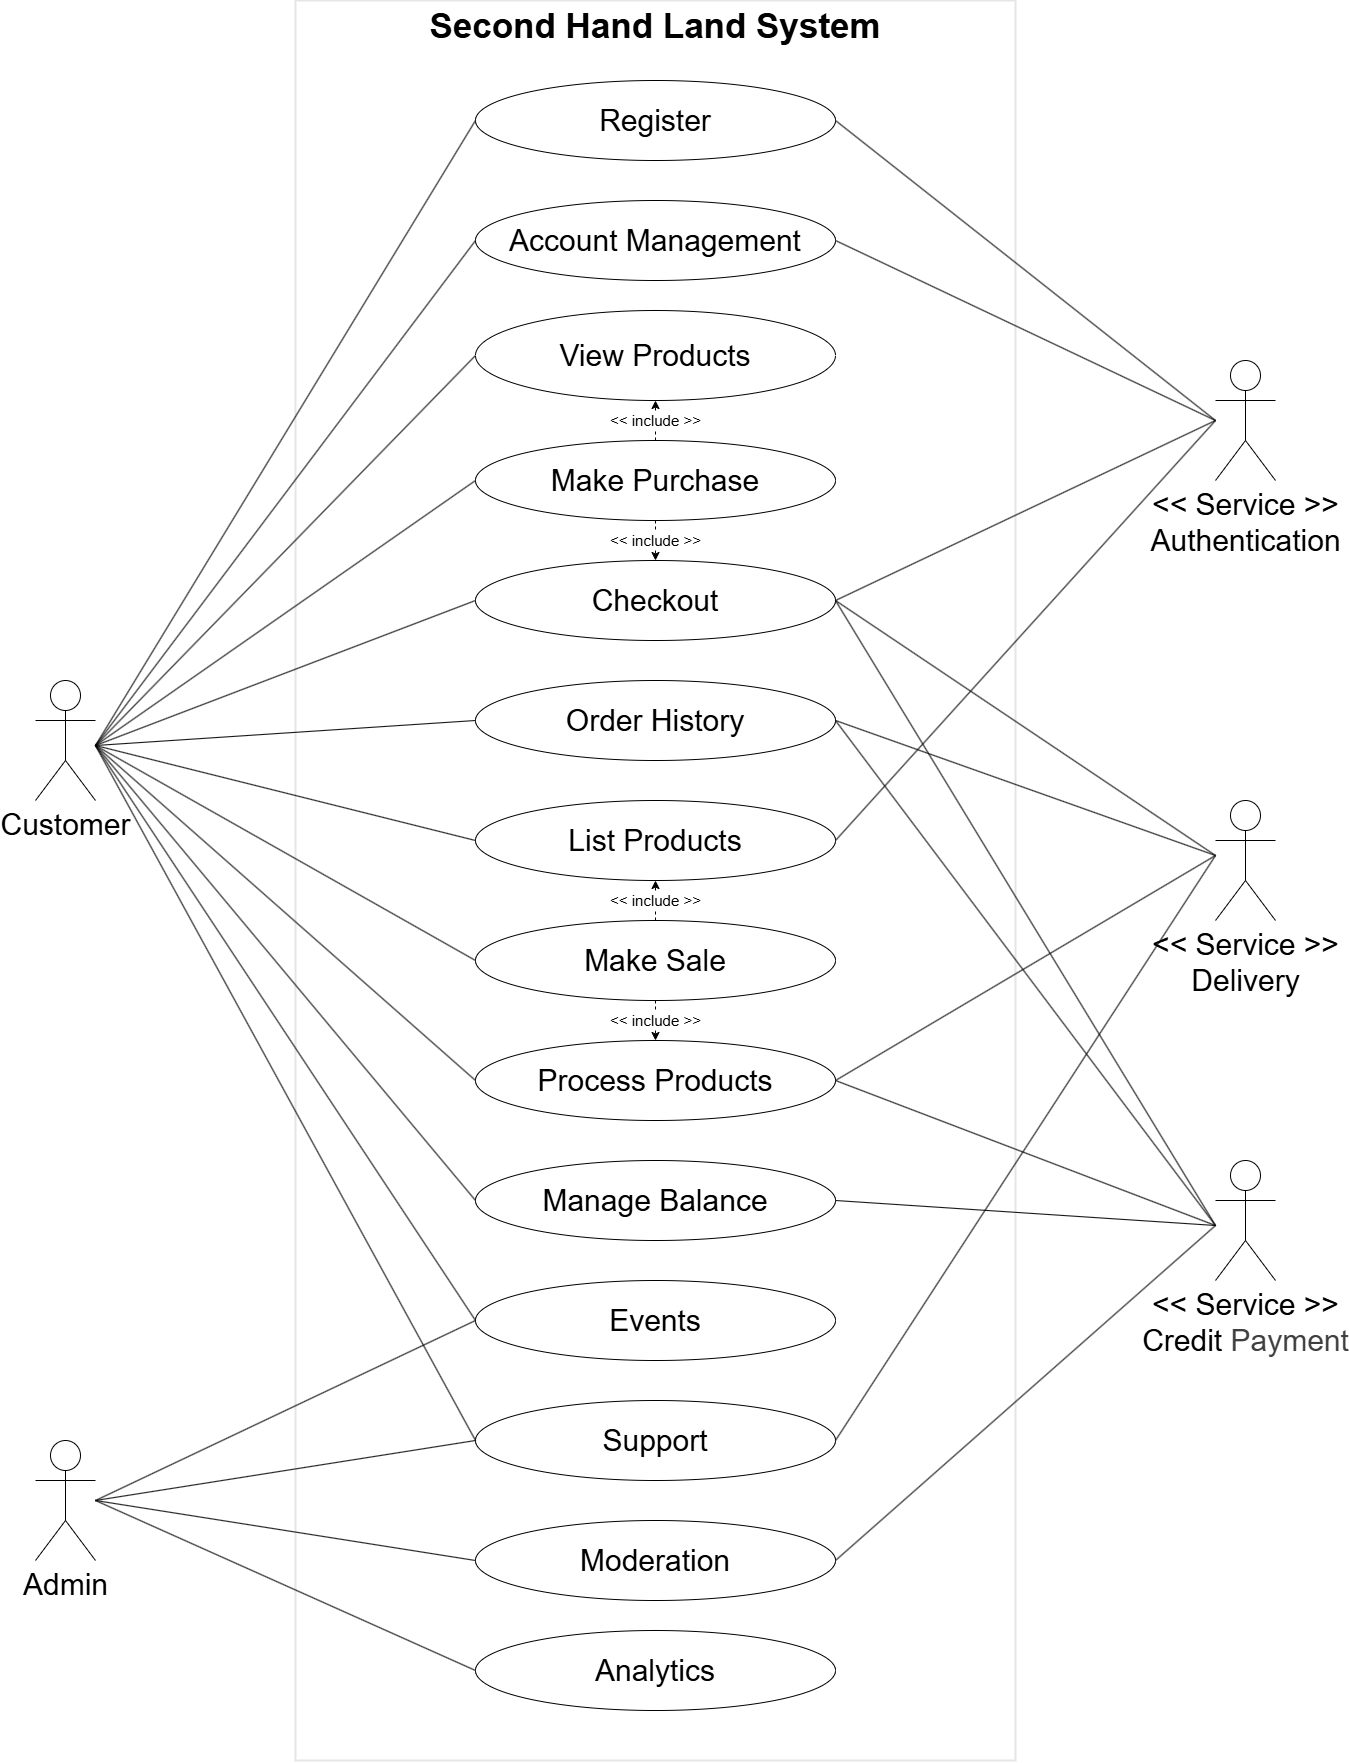
\includegraphics[width=0.7\textwidth]{../usecases/system/system.drawio.png}
    \caption{Sơ đồ Use Case}
    \label{fig:usecase}
\end{figure}


\subsection{Mô tả Use Case}

\label{LastPageArabic}
\end{document}

